
\chapter{Supplementary Notes}
  
  \section{Chemistry}
    
    \cite{Patchen2007} examine the branching step where isoprene either forms ROO or RONO$_2$, and for specific conditions they determine the reaction rates for each branch.
    They find the most frequent pathway is the formation of ROO (99.3\%).
    Although the nitrates formation is relatively infrequent, this pathway can lead to NO$_X$ transport into clean environments (\cite{Horowitz1998}).
    This transport can be exacerbated by fast winds and low OH concentrations, making nitrates an important factor in modelling atmospheric chemistry.
    
    PAN has a relatively long lifetime (against OH, order of 1 day) and is able to transport and release the NO$_X$ in environments which are quite far from any emissions.
    
    \subsubsection{SOA}
    \label{LR:VOCs:IsopCascade:SOA}
    
    SOA formation from VOCs in atmospheric CTMs is generally imperfect due to the complicated chemistry and diverse nature of atmospheric conditions.
    Yields of SOA from VOCs are often lumped together and based on empirical laboratory chamber data. 
    VOC oxidation was not feasible $\sim 13$ years ago (2005), as chamber studies did not extend over a large enough parameter range and the importance of heterogeneous aerosol chemistry on SOA formation was unquantified \citep{Kanakidou2005}.
    
    
    %% SOA production and overview?
    Gas phase emissions with higher vapour pressures can be oxidised into lower vapour pressure products which will partition between gas and particle phase, often called semi or non-volatile. 
    The aerosol products from these gas phase emissions (or the children thereof) are called SOA \citep{Kanakidou2005}.
    In the \cite{Kanakidou2005} review of global SOA science, uncertainty in radiative forcing of aerosols is highlighted, and 20-90~\% of PM mass in the lower troposphere is OA.
    Less volatile OA also plays a role, although PM production from this source is complicated and makes up only a small fraction ($\sim 1 \%$) of the resulting PM (\cite{Kroll2008, Bei2012}).
    Modelling OA has many uncertainties due to the complexity of SOA formation and various pathways such as aqueous phase oxidation which can significantly contribute to concentrations.
    This is further hindered by poor understanding of precursor emissions, and lumping together various compounds, of which only some form SOA (for example ORVOCs in GEIA (back in 2005)).
    Satellite data requires SOA models to estimate a full vertical profile of aerosols for remote sensing techniques \citep{Kanakidou2005}.
    
    SOA formation from VOCs in atmospheric CTMs is generally imperfect due to the complicated chemistry and diverse nature of atmospheric conditions.
    Yields of SOA from VOCs are often lumped together and based on empirical laboratory chamber data. 
    VOC oxidation was not feasible $\sim 13$ years ago (2005), as chamber studies did not extend over a large enough parameter range and the importance of heterogeneous aerosol chemistry on SOA formation was unquantified \citep{Kanakidou2005}.
    
    One of the large uncertainties with OA is the total effect on radiative forcing, 12 years ago it was well understood that most OA cool the atmosphere, with smaller particles having a larger affect due to the size matching the wavelengths of visible light \citep{Kanakidou2005}. 
    Transport and indirect effects complicate matters further, with cloud creation and modification of cloud properties being quite difficult to accurately predict.
    In the third IPCC report \citep{IPCC2001}, the uncertainty involved if OA forcing was a factor of 3 times the estimated effect. 
    This has since been improved however OA and cloud formation still remains a large uncertainty in more recent IPCC reports \citep{IPCC_Chapter2}.
    Figure \ref{LR:VOCs:IsopCascade:SOA:fig_IPCC_RF_AR4} shows the radiative forcing (RF) of various atmospheric constituents, it's clear that OA uncertainty dominates.
    Figure \ref{LR:VOCs:IsopCascade:SOA:fig_IPCC_RF_AR5} shows the same summary updated in chapter 8 of the fifth report, where the SOA uncertainty remains quite large.
    It's currently understood that SOA plays an indirect and complex role in cloud properties, with a net cooling effect \citep[Chapter 7,8]{IPCC_AR5_WG1}
    
    \begin{figure}
      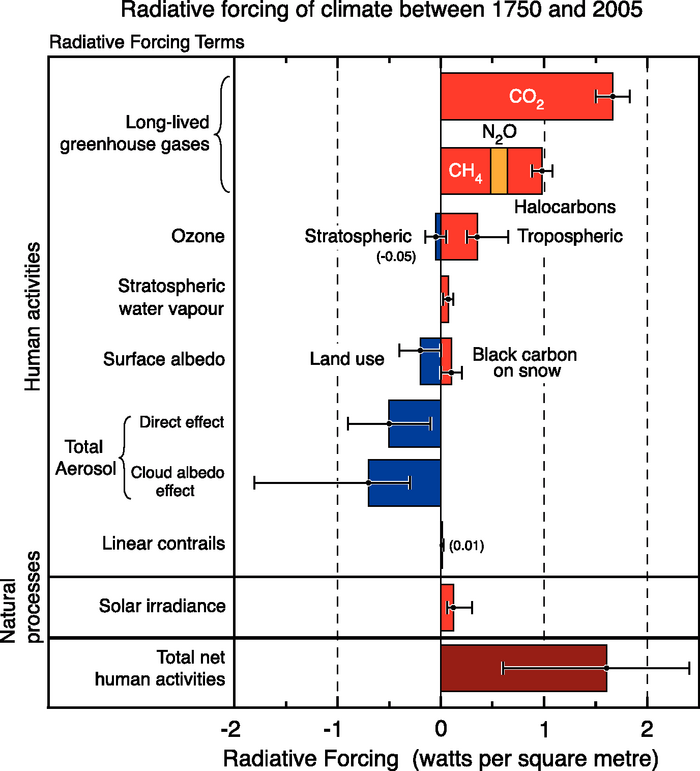
\includegraphics[width=\textwidth]{Figures/IPCC_WG1AR4_RFSummary.png}
      \caption{%
        The overall radiative forcings and uncertainties of several atmospheric constituents
        This is an image taken from \cite{IPCC_Chapter2}, found at \url{https://www.ipcc.ch/publications_and_data/ar4/wg1/en/faq-2-1.html}.}
      \label{LR:VOCs:IsopCascade:SOA:fig_IPCC_RF_AR4}
    \end{figure}
    
    \begin{figure}
      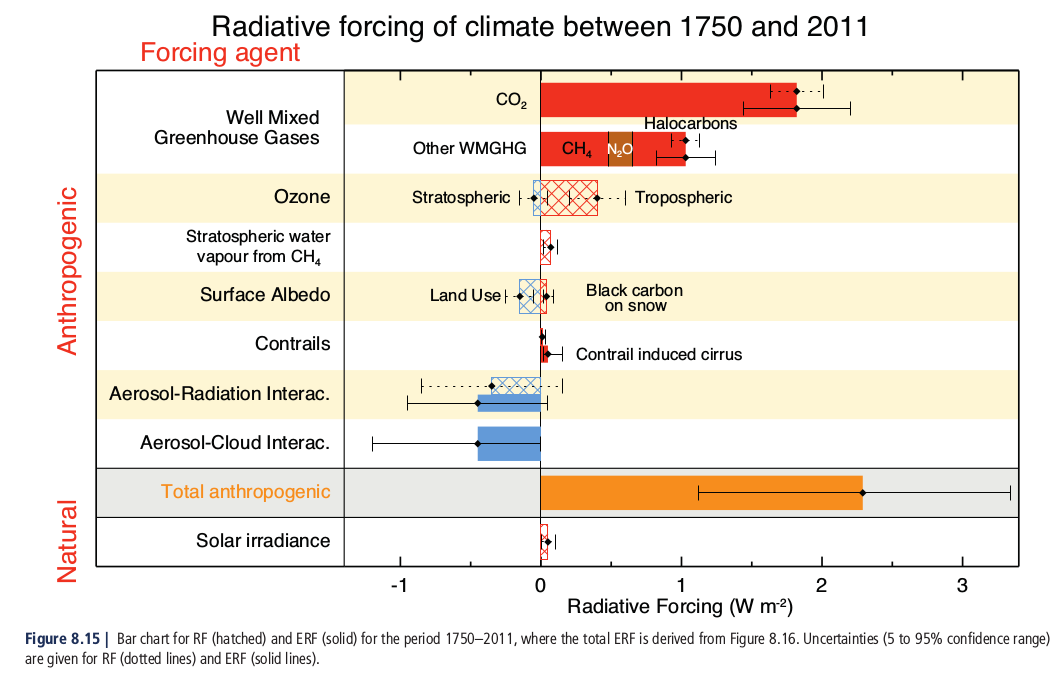
\includegraphics[width=\textwidth]{Figures/IPCC_WG1AR5_RFSummary.png}
      \caption{%
        The overall radiative forcings and uncertainties of several atmospheric constituents
        This is an image taken from \cite{IPCC_AR5_WG1}, chapter 8.}
      \label{LR:VOCs:IsopCascade:SOA:fig_IPCC_RF_AR5}
    \end{figure}    
    
    (TODO: read more of Kanakidou2005)
    The emissions of precursors to SOA was and is quite uncertain, in \cite{Kanakidou2005} they state that these uncertainties range from a factor of 2 to 5.
    They highlight emissions and flux measurements as well as implementing satellite data in models as a means of improving the emissions inventories.
    In 2005, (as of \cite{Kanakidou2005},) the knowledge gaps in isoprene and terpene oxidation processes included precursor gases to SOA, impact of NO$_X$ on SOA formation, heterogeneous reactions between particles and gaseous compounds, aqueous phase chemistry, and complete aerosol compositions.
    At this time SOA driven nucleation was under debate, as chamber studies showed that SOA led to new particles but only in the particle free laboratory setting. 
    Nucleation of new particles was suppressed by condensation if any seed aerosol was already present.
    Observed nucleation outside of laboratories was suggested to have arisen from biogenic SOAs, driven by ozonolysis.
    \cite{Kanakidou2005} concluded that it is very likely that organics contribute to particle growth and formation rates.
    
    
  \subsection{Relationship to Glyoxyl TODO: remove if never used}
    
    Another chemical retrievable from satellite observation is Glyoxyl, which can be used to further determine what sort of precursors to HCHO are being emitted \citep{Stavrakou2009, Miller2014, Miller2017}.
    TODO: go through 2014 paper and see if it's easy to retrieve, then email Dr. Chris Miller.
    For example \cite{Cao2018_discuss} recently used Glyoxyl measurements to improve understanding of biogenic and anthropogenic NMVOC emissions over China.
    This involved using a method pioneered by \cite{Stavrakou2009} TODO: get this cite and check method out.
    
    Glyoxyl (CHOCHO) is important to us as it shares many properties with HCHO, and may provide additional information in determining isoprene emissions.
    Glyoxyl is another product of VOC oxidation in the atmosphere, with isoprene being the main source globally.
    Under high NO$_X$ conditions, glyoxyl forms rapidly, similarly to HCHO.
    However, glyoxyl also forms in low NO$_X$ environments both slowly (through isoprene epoxydiols), and rapidly (through di-hydroperoxide dicarbonyl compound photolysation \citep{Crounse2013}.
    This process is similar to the proposed mechanisms for hydroperoxyaldehydes by \cite{Peeters2014} and carbonyl nitrates \citep{Muller2014}.
    Aromatics which are largely anthropogenic form glyoxyl quickly, while HCHO is produced slower, allowing determination of anthropogenic sources \citep{Cao2018_discuss}.
    
    HCHO has been used to estimate isoprene emissions (some examples in Section \ref{LR:HCHO:SatelliteInversion}) but many uncertainties exist.
    One of these uncertainties is the yield of HCHO from isoprene, especially in low NO$_X$ environments.
    Glyoxyl could prove complementary to HCHO in constraining isoprene emissions (TODO: Read and cite Vrekoussis2009,2010, Chan Miller 2014, Alvarado 2014) \citep{Miller2017}.
    Recently \cite{Miller2017} updated GEOS-Chem to include the prompt formation of glyoxyl and compared this with satellite and airplane measurements over the USA.
    With coming geostationary satellites, which provide greater time resolved measurements of HCHO and CHOCHO, this mechanism could be used to clearly show when low NO$_X$ isoprene chemistry is being undertaken \citep{Miller2017}.